\chapter{System Testing and Analysis}
With the system fully designed, the next step is to confirm that all systems are operating correctly.
There were several methods used to confirm all these results, including unit tests, inspection via the debugger, and simple test programs to confirm functionality on hardware.

\section{SD Testing}

\paragraph{}
The first part of this project that needed to be tested was the creation and writing of files on the SD card.
To do this, a simple test program creating a csv file with dummy data was made.
During this testing, there were several issues discovered.
The first was that the STM32SD library does not define the function f\_unmount even though it is used in the library.
This function is typically a wrapper around f\_mount and passing in 0's for the filesystem and option.
By updating the f\_unmount function call to a f\_mount with the added parameters, the library worked fine.

\paragraph{}
After the issue with the library was resolved, the next issues were related to the hardware.
The pinout for the SDIO interface had some conflicts, resulting in the SD card being connected to non-SDIO pins.
This issue required a re-spin of the hardware to fix, delaying testing by several weeks.
During this time, attempts were made to rework the PCB to connect the SD card to the correct microcontroller pins.
It was discovered while attempting to run the test program that there were stability problems with the reworked connections.
There were a few instances where the SD object would initialize properly, indicating that the library was working successfully.
Once the re-spun board arrived, it was confirmed that the SD library was functional and the test program successfully created a dummy csv file shown in \cref{fig:CSVTest}.

\begin{figure}[H]
	\centering
	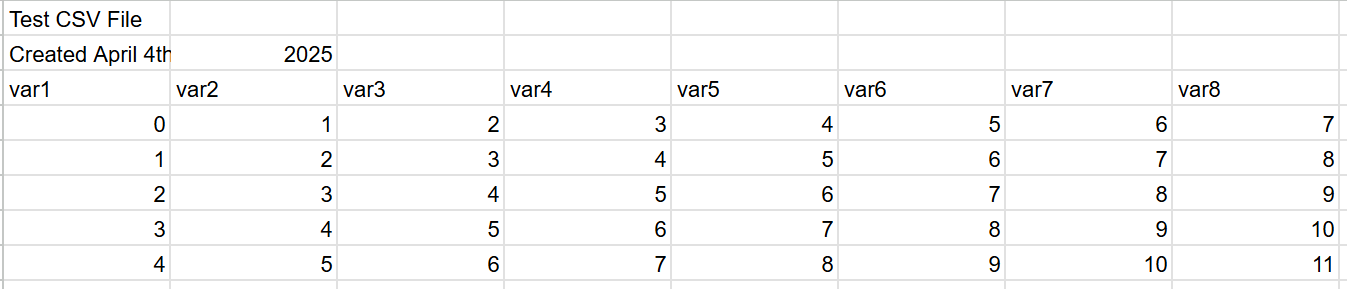
\includegraphics[width=\linewidth]{CSVTest.png}
	\caption{Dummy CSV file created on SD card}
	\label{fig:CSVTest}
\end{figure}

\section{Checksum Testing}

\paragraph{}
To confirm that the checksum calculation used in logging and radio communication was functioning as expected, a unit test was created.
There were 5 different values tested, and the checksum was computed by hand and then compared to what was calculated by the DAQ.
As can be seen in \cref{tab:ChecksumTesting}, the checksum was computed correctly in all tests.

\begin{table}[H] \label{tab:ChecksumTesting}
\caption{Checksum Unit Testing Results}
\centering
\begin{tabular}{c c c c}
\hline\hline
Test & Value & Hand Computed & DAQ Computed \\ [0.5ex]
\hline
1 & 0x0 & 0 & 0 \\
2 & 0xAFAFAFAFAF & 2625 & 2625 \\
3 & 0x123456789ABCDEF & 4432 & 4432 \\
4 & 0xF000 & 240 & 240 \\
5 & 0xFFFFFFFF & 2550 & 2550 \\ [1ex]
\hline
\end{tabular}
\end{table}

\section{Metadata Testing}

\paragraph{}
Metadata generation for files is a critical feature for being able to properly decode the data into something useful for design engineers to use.
To confirm that the metadata is being generated properly, the file metadata must first be computed by hand.
Then, since the SD card functionality has been confirmed to work previously, the file metadata can be written to a file on the SD card.
This file can be viewed in a hex editor to see each byte of the file, where it was confirmed to match the metadata generated by hand.

\paragraph{}
After confirming that the metadata section of the file is being written correctly, it needed to be confirmed that data was also being written to the file correctly.
To confirm this, dummy data can be written for a chunk of data that corresponds to each data section ID.
By inspecting the data written to the file, it can be confirmed that the data was written correctly and that the correct number of bytes was written.
This can also be done by inspecting a file in a hex editor.

\section{CAN Testing}

\paragraph{}
Two parts of CAN that needed to be tested.
The first was that two or more CAN nodes were able to communicate, or that the DAQ was able to communicate with any other node.
To accomplish this, another system designed for the Baja car was used.
These two boards were wired together, and a CAN test program was written to confirm that both transmitting and receiving were fully functional.
To start, an internal loopback test was performed, followed by an external loopback test, and finally completing a normal test between two nodes.
This test was completed by using a fixed ID of 1, a data length of 32 bytes, and the data section was filled with incrementing values starting from 0 and ending at 31, with each value corresponding to the index of the byte array of the message.

\paragraph{}
After the CAN bus was confirmed to work and data was transmitted, CAN loading also needed to be tested.
This could be done empirically, knowing the total amount of data being transmitted in each message and the frequency at which each message was being sent.
To confirm that the desired throughput was actually achieved, the total number of each CAN ID was tracked over 10 seconds to confirm that the correct number of CAN messages were being received.

\begin{table}[H] \label{table:CANTesting}
\caption{CAN Testing Results}
\centering
\begin{tabular}{c c c c c c}
\hline\hline
Message & Frequency & Data & 1 second & 5 seconds & 10 seconds \\ [0.5ex]
\hline
1 & 400 hz & 36 Bytes & 400 & 2000 & 4001 \\
2 & 400 hz & 48 Bytes & 400 & 2000 & 4001 \\
3 & 400 hz & 48 Bytes & 400 & 2000 & 4001 \\
4 & 100 hz & 8 Bytes & 100 & 500 & 1000 \\
5 & 10 hz & 16 Bytes & 10 & 50 & 100 \\
6 & 10 hz & 8 Bytes & 10 & 50 & 100 \\
7 & 100 hz & 20 Bytes & 100 & 500 & 1000 \\ [1ex]
\hline
\end{tabular}
\end{table}

\paragraph{}
As can be seen in \cref{table:CANTesting}, the CAN bus was not overloaded.
This is the expected result and supports the previously computed CAN loading and confirms that there are no issues with the amount of data being transmitted.
Additionally, this implies that there is room for additional nodes to send data, leaving room for different sensor expansions for permanent or temporary sensing units.

\section{Radio Testing}

\paragraph{}
The last system to test was radio communication.
To test that this task is working as expected, the Digi XTCU tool can be used to read all the data received over the air.
To confirm correct operation, a similar test used in the CAN testing was performed, where several bytes were written to the transmitting radio with incrementing values.
On the receiving side, these bytes can be viewed in the XTCU tool, confirming that all bytes being sent were received.

\paragraph{}
After confirming that all bytes being transmitted were being sent and received properly, the packet construction needed to be confirmed.
Since the checksum calculation was confirmed previously, the packet creation can be confirmed in the debugger.
On one iteration, a packet was constructed by hand and then confirmed by utilizing the debugger and looking at the bytes of the created packet.
It was confirmed that packets were being constructed correctly.

\paragraph{}
Finally, the radio's line of sight distance was tested.
This was done by driving the DAQ further and further away from the base antenna until no packets were received at the base side.
The base side remained at the aerospace hangar on campus (Bldg. 004) while the car was driven further down Highland Dr, and performance was measured at varying distances.
As can be seen from \cref{table:RadioDistance}, as the distance increased, the number of dropped packets also increased.
Once the car got 2.5 miles away, the number of packets being dropped became unacceptable.
This testing was done with as close to line of sight as was possible, but there were no fully clear lines of sight going as far as needed, so there are some interferences due to trees and elevation change.

\begin{table}[H] \label{table:RadioDistance}
\caption{Radio Distance Testing Results}
\centering
\begin{tabular}{c c c}
\hline\hline
Distance (mi) & Packets Dropped (\%) & Acceptable (Y/N) \\ [0.5ex]
\hline
1 mile & 12\% & Y \\
1.5 miles & 20 \% & Y \\
2 miles & 33 \% & Y \\
2.5 miles & 85 \% & N \\
3 miles & 100 \% & N \\ [1ex]
\hline
\end{tabular}
\end{table}

\section{System Testing}

\paragraph{}
Finally, everything was tested together to confirm that the system was behaving as expected.
This testing was performed on the car with two other nodes on the CAN bus, with the car idling for 10 minutes.
The reason for performing system testing on the car was to have real data that could be collected and compared back to what the system was truly doing to confirm that data was being logged correctly and transmitted over the radio without issue.
During this time, all data was logged with no known issues.
After testing the system in the aerospace hangar, the DAQ system was tested at a vehicle testing day to confirm that during normal vehicle operation, no new issues arose.
This test was done while the car was driving over the course of 4 hours, mimicking a competition endurance worth of testing.
During this test, there were no issues with logging data or radio communication.
From all of this testing, it is clear that the system is performing adequately and will be fully capable of logging data throughout testing and competitions.
